\documentclass[11pt]{article}

    \title{\textbf{Rapporto tecnico}}
    \author{Vincenzo Imperati 1834930}
    \date{}
    \usepackage{graphicx}
	\usepackage{float}
	\usepackage{hyperref}

\begin{document}

	\maketitle
	\thispagestyle{empty}


	\begin{abstract}
	In questo documento: viene descritto brevemente il sistema modellato; vengono descritti gli scenari operativi, come essi sono stati modellati e viene intuitivamente verificato e validato il modello; viene descritta brevemente l'architettura di sistema e come è stata modellata; vengono descritti i requisiti di sistema (funzionali e non funzionali) e come sono stati modellati; vengono descritti i risultati sperimentali ottenuti dagli script \textit{run.mos}, \textit{verify.py} e \textit{synth.py}.
	\end{abstract}

	\newpage
	\tableofcontents
	
	\newpage
	\section{Descrizione del sistema}
	Il sistema nel suo insieme permette:
	\begin{itemize}
		\itemsep0em
		\item alle aule di cambiare la loro agibilità (agibile, parzialmente agibile, inagibile) e di conseguenza la loro capienza. Dalla capienza dell'aula dipendono i posti ancora prenotabili dagli studenti. Se un'aula aumenta la sua capienza dopo il cambio di stato, ci saranno più posti prenotabili; ma se avviene il contrario ce ne saranno di meno, o addirittura verranno cancellate le ultime prenotazioni effettuate per non eccedere la capienza;
		\item agli studenti di poter effettuare la prenotazione di un posto in aula o di cancellarla. La richiesta di effettuare una prenotazione va a buon fine se, nell'aula di cui la prenotazione fa riferimento, vi sono ancora posti liberi. La richiesta di cancellazione va a buon fine se lo studente aveva già effettuato la prenotazione corripsondente;
		\item tramite un sottosistema di gestire per ogni aula le prenotazioni effettuate;
		\item tramite il GOMP di aggregare le informazioni del sistema per poterle mostrare quando richiesto dall'interfaccia Prodigit;
		\item tramite l'interfaccia Prodigit di richiedere e visualizzare le informazioni del sistema;
		\item tramite dei monitor di controllare la correttezza e la coerenza delle interazioni tra le parti.
	\end{itemize}
	
	\newpage
	\section{Scenari operativi}
	Gli scenari possibili del sistema sono i seguenti:
	\begin{enumerate}
		\itemsep0em
		\item L'aula può cambiare la sua agibilità, quindi passare da uno stato all'altro tra i seguenti: \textit{aula agibile}, \textit{aula parzialmente agibile}, \textit{aula inagibile}. L'aula agibile ha la massima capienza disponibile, l'aula parzialmente inagibile ha una capienza ridotta, l'aula inagibile ha capienza pari a zero;
		\item Lo studente se non ha ancora effettuato una prenotazione per una data aula, può effettuare la prenotazione;
		\item Lo studente se ha già effettuato una prenotazione per una data aula, può cancellare la prenotazione
		\item Il sottosistema per le prenotazioni aggiorna constantemente il numero di posti ancora disponibili per ogni aula, e quindi accetta o rifiuta le richieste di effettuazione e cancellazione delle prenotazioni. Il sottosistema ha il compito di non mandare in underflow o overflow le liste delle prenotazioni delle aule; e di eccettare qualsiasi prenotazione se vi sono dei posti disponibili. Il sottosistema ha anche il compito di ridimensionare la lista delle prenotazioni dell'aula qualora questa cambi di stato; e ha anche il compito di svuotare le liste delle prenotazioni delle aule qualora l'evento di cui sono state fatte le prenotazioni termina;
		\item Il GOMP aggrega constantemente tutte le informazioni del sistema. Propio per questo motivo potrebbe non performare come dovrebbe e quindi potrebbe andare in \textit{down} invece che essere \textit{operativo}. Se il GOMP è in down, quest'ultimo non conoscerà le informazioni correnti in circolo nel sistema e quindi avrà una vecchia versione di queste. Qualora l'interfaccia Prodigit interrogasse il GOMP per chiedere le informazioni, quest'ultimo quindi mostrerà la vecchia versione delle informazioni, e quindi l'interfaccia riceverà delle informazioni non completamente coerenti con lo stato corrente del sistema;
		\item L'interfaccia Prodigit richiede al GOMP le informazioni correnti del sistema. Per avere una copia esatta delle informazioni del sistema, l'interfaccia Prodigit dovrebbe interrogare il GOMP costantemente, e questo comporterebbe un dispendio di energia ingiustificato qualora le informazioni non cambino in modo repentino e consistentemente. D'altro canto chiedere informazioni poco frequentemente potrebbe generare un elevata inconsistenza dei dati in confronto a quelli correnti nel sistema;
		\item Il monitor non funzionale ha il compito di monitorare la correttezza dell'operato del sottosistema di prenotazione;
		\item Il monitor non funzionale ha il compito di monitorare che i dati posseduti dall'interfaccia Prodigit non superino una soglia massima di incoerenza con i dati correnti del sistema.
	\end{enumerate}
	
	\newpage
	\section{Architettura di sistema}
	Di seguito vengono descritte le componenti del sistema e viene spiegato come sono state modellate, ottenendo in fine una convincente ed esauriente dimostrazione di completezza e correttezza del sistema modellato:
	\begin{description}
		\addtolength{\itemindent}{0.5cm}
		\itemsep0em
		\item [Aule] agenti esterni al sistema che comunicano la loro agibilità e la loro capienza. Possono ospitare eventi prenotabili dagli studenti fino al momento di inizio dell'evento in questione.
		\begin{itemize}
			\itemsep0em
			\item Il modello contiene una sola aula (il ragionamento è analogo per modellare più aule contemporaneamente). L'aula è modellata in un \textit{block}, il quale passa le informazioni dell'aula al GOMP e al sottosistema di prenotazione. Il cambio di agibilità dell'aula avviene tramite una catena di Markov, e i cambi di stato avvengono ogni 6 ore. La frequenza di cambio di stato e le probabilità nella catena di Markov, sono dati modificabili e quelli di default sono stati impostati ragionevolmente;
		\end{itemize}
		\item [Studenti] agenti esterni che comunicano le loro richieste (effettuazione o cancellazione prenotazione) al sottosistema di prenotazione. Si assume che le richieste risppettino i vincoli logistici citati precedentemente (il sistema e il modello dunque non approfondiscono questi vincoli e assumono che vengano sempre rispettati).
		\begin{itemize}
			\itemsep0em
			\item Il modello contiene un solo gruppo di studenti che fanno richieste per lo stesso evento (il ragionamento è analogo per modellare più gruppi di studenti che fanno richieste per più eventi). Gli studenti sono modellati in un \textit{block}, il quale passa ogni momento (ogni minuto) le nuove richieste al sottosistema di prenotazione. Il numero delle nuove richieste degli studenti viene calcolato con una distribuzione di probabilità. La distribuzione è modificabile e quella di default è impostata ragionevolmente;
		\end{itemize}
		\item [Sottosistema di prenotazione] agente interno che riceve per ogni evento la capienza dell'aula e le nuove richieste per l'evento. Il sottosistema ha in memoria i posti occupati per ogni evento, che quindi deve aggiornare correttamente. Il sottosistema ha anche il compito di svuotare i posti occupati per gli eventi appena terminati, oppure perchè l'aula è diventata inagibile.
		\begin{itemize}
			\itemsep0em
			\item Il modello contiene un sottosistema di prenotazione che gestisce un solo evento (il ragionamento è analogo per modellare un sottosistema di prenotazione che gestisce più eventi). Il sottosistema è modellato in un \textit{block}, il quale passa ogni momento (ogni minuto) il numero di posti prenotati per l'evento al GOMP. Il nuovo numero di posti occupati viene viene aggiornato rispettando tutti i requisiti precedentemente descritto;
		\end{itemize}
		\item [GOMP] agente interno che aggrega le informazioni del sistema e le comunica all'interfaccia Prodigit quando le richiede. Il GOMP comunica le informazioni correnti all'interfaccia Prodigit, quando il primo è operativo. Quando il GOMP non è operativo comunica le ultime informazioni valide che aveva aggregato.
		\begin{itemize}
			\itemsep0em
			\item Il modello contiene un GOMP che aggrega le informazioni che ruotano intorno ad un solo evento (il ragionamento è analogo per modellare un GOMP che aggreghi informazioni che ruotano intorno a più eventi). Il GOMP è modellato in un \textit{block}, il quale passa le informazioni aggregate all'interfaccia Prodigit. Il cambio di stato (in down, operativo) del GOMP avviene tramite una catena di Markov, e i cambi di stato avvengono ogni momento (ogni minuto). La frequenza di cambio di stato e le probabilità nella catena di Markov, sono dati modificabili e quelli di default sono stati impostati ragionevolmente;
		\end{itemize}
		\item [Interfaccia Prodigit] agente interno che interroga il GOMP per richiedere i dati correnti del sistema. Può ottenere come risposta i dati correnti qualora il GOMP sia operativo, o dati non correnti qualora il GOMP sia in down.
		\begin{itemize}
			\itemsep0em
			\item Il modello contiene un'interfaccia Prodigit che richiede le informazioni che ruotano intorno ad un solo evento (il ragionamento è analogo per modellare un'interfaccia Prodigit che richiede le informazioni che ruotano intorno a più eventi). L'interfaccia Prodigit è modellata in un \textit{block}, il quale richiede le informazioni al GOMP. La frequenza delle richieste al GOMP è impostata ragionevolmente al fine di massimizzare la funzione obiettivo del requisito non funzionale;
		\end{itemize}
		\item [Monitor funzionale] agente interno che monitora i requisiti funzionali del sistema. Questi ultimi sono relativi alla correttezza dell'operato del sottosistema di prenotazione.
		 \begin{itemize}
			\itemsep0em
			\item Il modello contiene un monitor funzionale che monitora la correttezza dell'operato del sottosistema. Il monitor funzionale è modellato in un \textit{block}, il quale richiede le informazioni necessarie per il monitoraggio che avviene ogni momento (ogni minuto);
		\end{itemize}
		\item [Monitor non funzionale] agente interno che monitora i requisiti non funzionali del sistema. Questi ultimi sono relativi alla consistenza dei dati che riceve l'interfaccia Prodigit.
		 \begin{itemize}
			\itemsep0em
			\item Il modello contiene un monitor non funzionale che monitora la consistenza dei dati che riceve l'interfaccia Prodigit. Il monitor non funzionale è modellato in un \textit{block}, il quale richiede le informazioni necessarie per il monitoraggio che avviene ogni momento (ogni minuto).
		\end{itemize}
	\end{description}
	
	\newpage
	\section{Requisiti di sistema}
	Il sistema rispetta i seguenti requisiti funzionali monitorati dal monitor funzionale:
	\begin{description}
		\addtolength{\itemindent}{0.5cm}
		\itemsep0em
		\item [Safety] le liste delle prenotazioni non vanno mai in underflow o in overflow;
		\item [Liveness] finchè ci sono posti disponibili per gli eventi, le richieste di prenotazione non vengono rifiutate.
	\end{description}
	Il sistema rispetta i seguenti requisiti non funzionali monitorati dal monitor non funzionale:
	\begin{description}
		\addtolength{\itemindent}{0.5cm}
		\itemsep0em
		\item [Minima richiesta, massima congruenza dei dati] è nota la frequenza con cui l'interfaccia Prodigit deve richiedere i dati al GOMP a finchè la funzione obiettivo in \textit{synth.py} è massima.
	\end{description}

	
	\newpage
	\section{Risultati sperimentali}
	Di seguito la descrizione dei tre script:
	\begin{description}
		\addtolength{\itemindent}{0.5cm}
		\itemsep0em
		\item [run.mos] script che se eseguito simula il modello del sistema precedentemente descritto;
		\item [verify.py] script che se eseguito verifica che il modello del sistema rispetta i requisiti funzionali. Prende in input il numero di samples da simulare, e le volte che questi devono essere simulati;
		\item [synth.py] script che se eseguito trova la frequenza che deve rispettare l'interfaccia Prodigit per soddisfare il requisito non funzionale. Prende in input il numero di samples da simulare, e la grandezza della griglia sulla quale trovare la migliore frequenza di richiesta.
	\end{description}
		
	\begin{figure}[H]
	\centering
	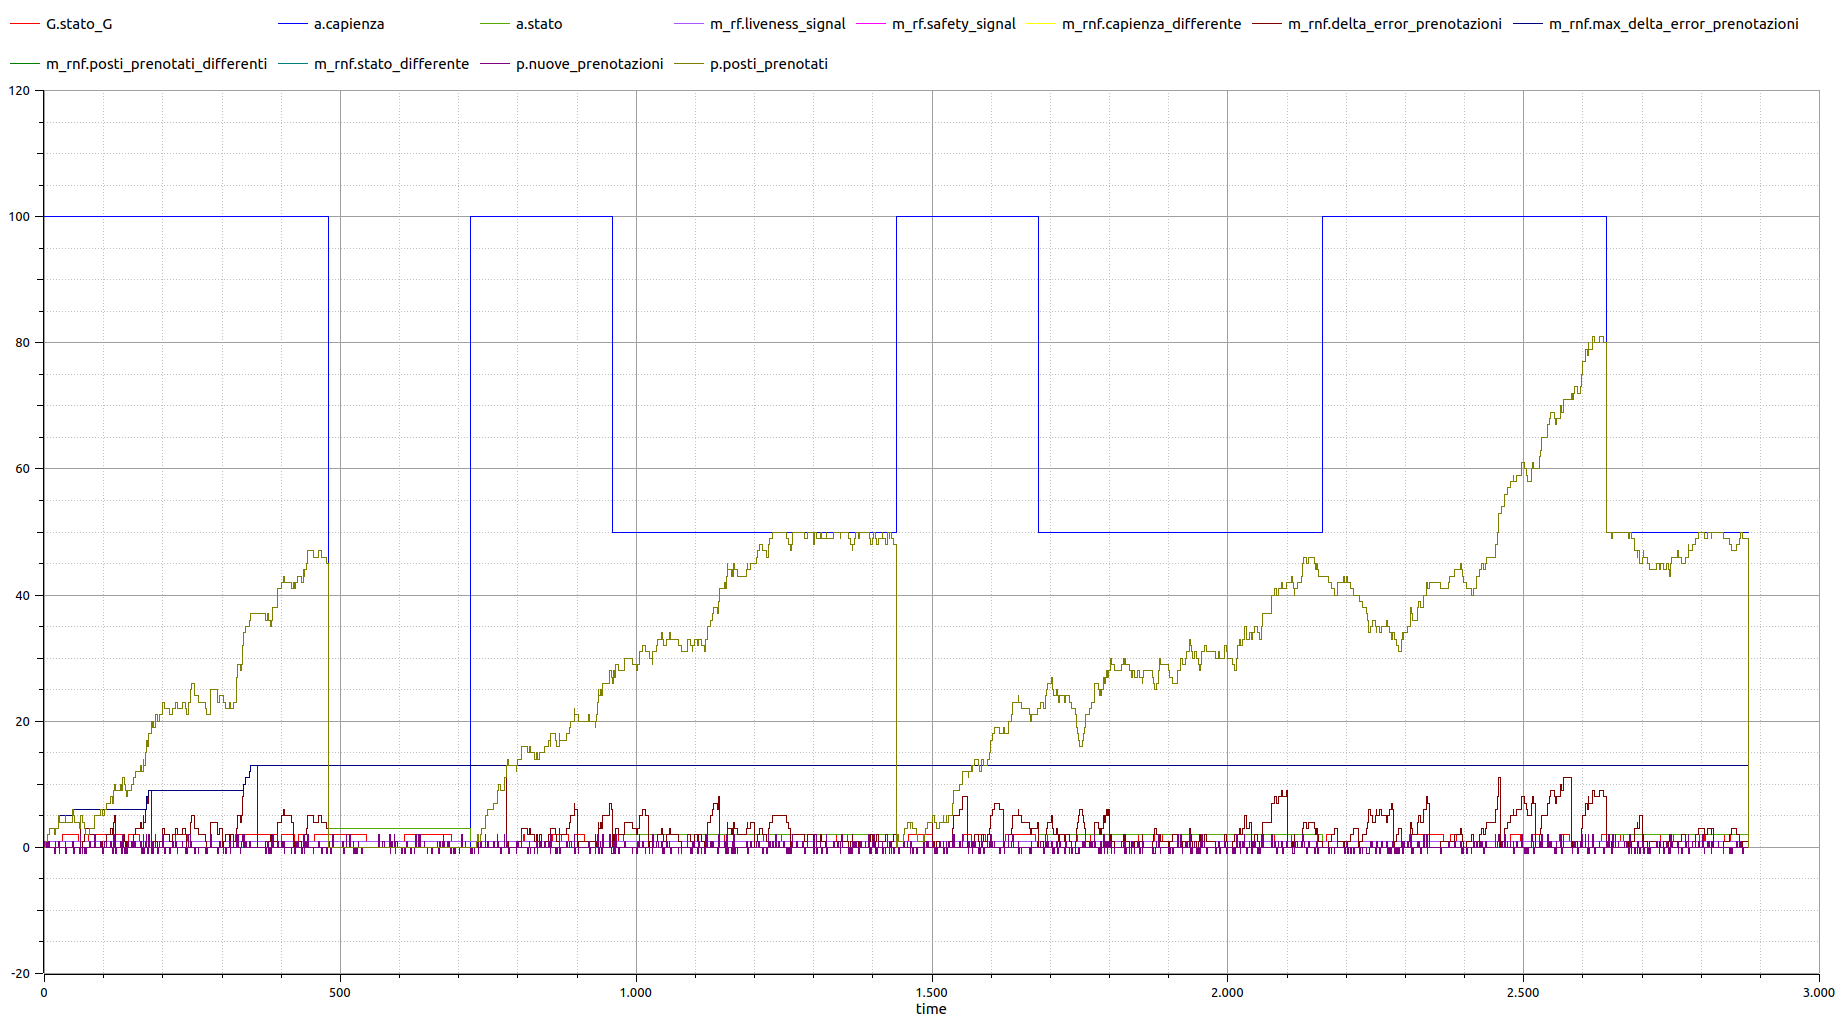
\includegraphics[width=1\textwidth]{Plot.png}
	\caption{Plot}
	\end{figure}
	

\end{document}
